\chapter{Experimentos}
\label{experimentos}
A lo largo de esta sección, se tratarán de forma detallada los distintos experimentos que se han realizado para este proyecto con el fin de 
poner en práctica los conocimientos obtenidos durante el proceso de investigación de la materia. Para cada experimento se planteará cuál es el 
objetivo a alcanzar y los posibles enfoques a aplicar para llegar a una solución, además de tratar los retos encontrados por el camino, los 
resultados del experimento y las lecciones que puedan ser aprendidas de este.

\section{Prueba de concepto Qiling}
\section{Fuzzing de un parser JSON}
\section{Identificación de vulnerabilidad real a través de fuzzing: Netgear R7000}
\subsection{Introducción al dispositivo}
El Netgear R7000, también conocido como Nighthawk AC1900 es un router WIFI ''inteligente'' lanzado al mercado originalmente en 2013 con una última
revisión del hardware en 2018 que sigue en venta actualmente. Este producto de la gama de routers premium de Netgear recibe actualizaciones periódicas
a día de hoy por parte del fabricante y se trata de una elección muy popular entre aquellos consumidores que buscan un router dual-band de altas prestaciones. 
\begin{figure}[H]
    \centering
    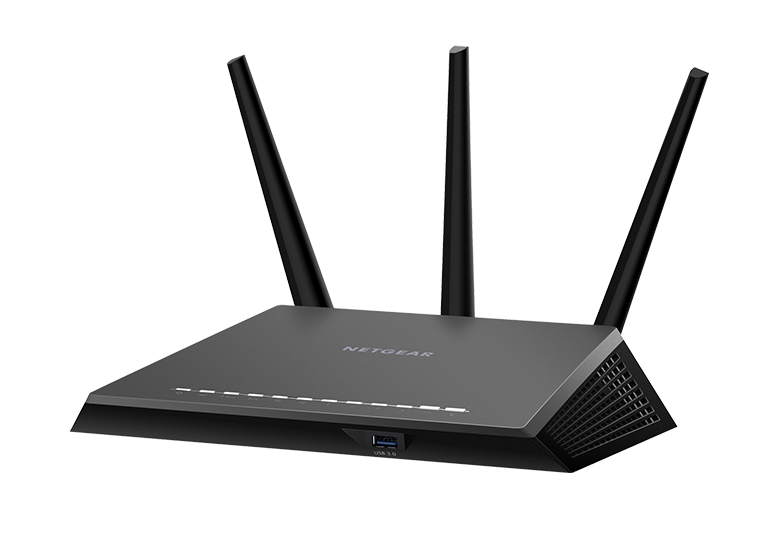
\includegraphics[scale=0.30]{r7000.png}
    \caption{Netgear R7000 (Nighthawk AC1900).}
    \label{fig:r7000}
\end{figure}

\subsection{Recopilación de información}
Consultando sus especificaciones técnicas principales 
encontramos que posee una CPU de 1GHz dual-core, 256MB de RAM, 128MB de memoria flash y soporte para dual-band de 2'4GHz a 600Mbps y de 5GHz a 
1300Mbps. Aunque estas especificaciones son interesantes a la hora de conocer las restricciones cómo de restringido en rendimiento es el dispositivo,
no son lo suficientemente detalladas como para aportarnos información clave que necesitamos conocer para aplicar emulación sobre el dispositivo.
Principalmente, desconocemos el procesador que está siendo utilizado y su arquitectura, ya que el fabricante no proporciona dicha información.
Cuando nos encontramos en esta situación en la que deseamos conocer información más detallada sobre los componentes internos de un dispositivo, 
una posible solución es consultar su informe de aceptación para la certificación del FCC [TBD REFERENCIA] en la base de datos \hyperlink{fccid.io}{fccid.io}.
El FCC es un organismo de certificación encargado de evaluar todo producto que vaya a ser comercializado en los Estados Unidos que emita 
radiofrecuencias con el fin de asegurar que dichos dispositivos no produzcan interferencias dañinas que pudieran afectar al correcto
funcionamiento de otros dispositivos como equipamiento médico, aeronáutico o sistemas de telecomunicaciones.\bigskip

Accediendo a la base de datos podemos encontrar información de los reportes que se han ido realizando sobre las distintas iteraciones del producto,
concretamente, el reporte de mayor interés para nuestra tarea es el titulado ''Internal Photos'' publicado para la revisión lanzada en 2018\cite{netgearFCCid}.
Buscando lo que pudiera ser la CPU principal nos llaman la atención dos chips mostrados en el informe. El primero (figura \ref{fig:r7000transceptor}), al 
consultar la ficha técnica del BCM4360 descubrimos que se trata de un transceptor WIFI del fabricante Broadcom, por lo tanto no es lo que tratamos de 
encontrar. Respecto al segundo chip (figura \ref{fig:r7000cpu}), consultando las especificaciones presentes en la ficha técnica del Netgear R7000 
(tabla \ref{table:r7000}) proporcionada por OpenWRT podemos ver que se trata de un System on a Chip (SoC) WIFI lanzado al mercado en 2013\cite{broadcomSOCs} 
que en su interior contiene un procesador dual core ARM Cortex A9 de 32 bits.

\begin{figure}[H]
    \centering
    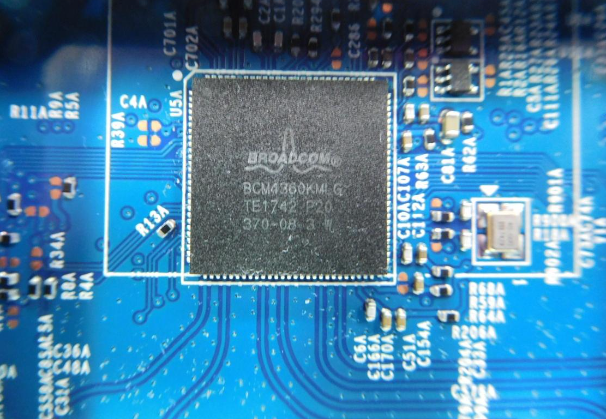
\includegraphics[scale=0.45]{r7000transceptor.png}
    \caption{Broadcom BCM4360 en el interior del Netgear R7000.\cite{netgearFCCid}}
    \label{fig:r7000transceptor}
\end{figure}

\begin{figure}[H]
    \centering
    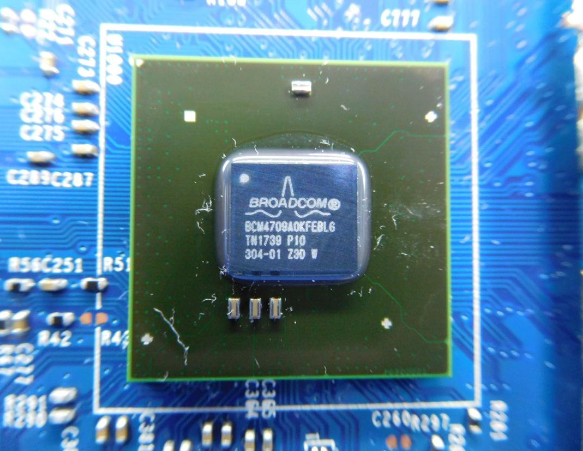
\includegraphics[scale=0.59]{r7000cpu.png}
    \caption{Broadcom BCM47 en el interior del Netgear R7000.\cite{netgearFCCid}}
    \label{fig:r7000cpu}
\end{figure}

\begin{table}[H]
    \centering
    \begin{tabular}{ |l|m{20em}| }
    \hline
    FCC ID                      & PY313200233                      \\\hline
    Industry Canada ID          & 4054A-13200233                   \\\hline
    Voltaje                     & 12 VDC, 3.5 A                    \\\hline
    CPU/SoC                     & Broadcom BCM4709A0 @1 GHz        \\\hline
    Arquitectura CPU            & ARM Cortex A9 (2 cores)          \\\hline
    Flash / RAM                 & 128 MiB / 256 MiB                \\\hline
    Chip WI1 \& WI2             & Broadcom BCM4360                 \\\hline
    Protocolos WI1 \& WI2       & an+ac / bgn                      \\\hline
    Configuración MIMO wireless & 3x3:3                            \\\hline
    Conector de antena          & U.FL, RP-SMA                     \\\hline
    Switch \& Ethernet          & Broadcom BCM4709A0               \\\hline
    Puertos WAN/LAN             & 1 / 4 (up to 1 Gb/s)             \\\hline
    Puertos USB                 & 1x USB 3.0, 1x USB 2.0           \\\hline
    Puerto serie                & 4-pin header, internal, 3.3V TTL \\\hline
    \end{tabular}
    \caption{Especificaciones del Netgear R7000.\cite{r7000datasheet}}
    \label{table:r7000}
\end{table}

Aunque Broadcom no proporciona una datasheet con las especificaciones del SoC, 
si que podemos consultar información más detallada sobre el Cortex A9 a través de la documentación oficial de ARM\cite{cortexA9}. Gracias a esto podemos 
conocer detalles como información sobre la Memory Management Unit (MMU) que utiliza la CPU. Esta información es de gran importancia ya que como explicaban
Muench et al.\cite{Muench2018}, la presencia de una MMU en un dispositivo empotrado puede alterar drásticamente el comportamiento de este ante corrupciones de 
memoria. Un dispositivo sin MMU puede no detectar fallas de memoria y seguir funcionando en un estado indefinido mientras que uno con MMU provoca un 
crash al detectar corrupción de memoria o la realización de alguna operación ilegal. Según la documentación oficial de la CPU, el procesador utiliza la MMU 
diseñada para la arquitectura Armv7, por lo que podemos deducir que un crash que encontremos aplicando fuzzing al firmware mediante emulación, podrá ser replicado
en el dispositivo real.

\subsection{Obtención del firmware}
Una vez hemos recopilado información sobre el objeto de estudio, necesitaremos conseguir el firmware del dispositivo para proceder a su análisis y posterior 
emulación. A la hora de conseguir el firmware de un dispositivo IoT podemos enfrentarnos a una serie de retos dependiendo de cómo el fabricante distribuya
las imágenes del firmware. Podemos categorizarlos de la siguiente mantera:
\begin{itemize}
    \item \textbf{Medio de distribución}: En el mejor de los casos, el fabricante provee un enlace de descarga del firmware a través de su portal de soporte oficial. Aunque
    este suele ser el caso para dispositivos como routers o cámaras IP, no es común en otros dispositivos aún más limitados como bombillas inteligentes o asistentes de voz.
    También hay fabricantes que con el objetivo de intentar evitar que usuarios puedan aplicar técnicas de ingeniería inversa sobre los paquetes de actualización, integran 
    todo el proceso de actualización a través de una app móvil o desde el propio dispositivo. Ante esto, es posible hacer uso de iptables para redirigir el tráfico
    de la aplicación o del dispositivo e intentar interceptar las peticiones al servidor de descargas de firmware. Por último, existe la posibilidad de que el fabricante no 
    haya provisto al dispositivo de un mecanismo de actualización para el usuario. Como último recurso, sería posible desmontar el dispositivo e intentar extraer el firmware 
    a través de la interfaz JTAG o leyendo los contenidos de la memoria FLASH utilizando un programador flash (figura \ref{fig:programador}).
    \begin{figure}[H]
        \centering
        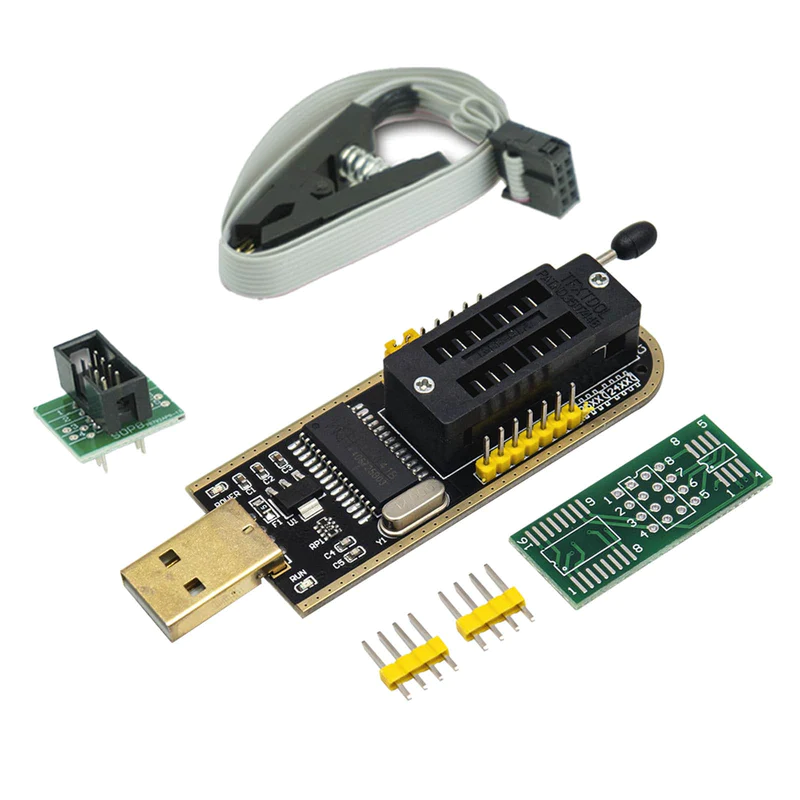
\includegraphics[scale=0.35]{programmer.png}
        \caption{Programador flash CH341A genérico.}
        \label{fig:programador}
    \end{figure}
    \item \textbf{Cifrado}: Además de no proporcionar un portal de descargas de firmware, los fabricantes también suelen cifrar sus paquetes de actualización para dificultar las 
    tareas de análisis e ingeniería inversa. Dicho firmware es posteriormente descifrado por la rutina de actualización del dispositivo. Cuando se da este caso desgraciadamente 
    solo quedan dos opciones, o extraer el firmware del mismo dispositivo como se ha comentado en el punto anterior o intentar obtener la versión del firmware previa a que el 
    fabricante implementara el cifrado en las actualizaciones y aplicar ingeniería inversa sobre la rutina de descifrado del firmware para llevar a cabo nuestra propia implementación. 
    \item \textbf{Formato}: Es bastante común para los fabricantes distribuir sus paquetes de firmware en formatos propietarios difíciles de tratar sin software especializado. 
    Binwalk\cite{binwalk} es una herramienta que puede ayudar con el análisis y desenpaquetado de imágenes firmware en binarios de los cuales se desconoce su estructura. El uso de esta herramienta
    será tratado a continuación. También es posible que se den casos en los que binwalk no sea capaz de identificar o extraer correctamente el contenido de la imagen firmware, 
    teniendo que recurrir al diseño de herramientas específicas para el firmware con el que se está trabajando, identificando los offsets a partir de dónde empiezan los distintos 
    componentes de este y extrayéndolos manualmente con herramientas como dd de las coreutils de GNU.
\end{itemize}

Para el Netgear R7000, es posible obtener el firmware a través de su \href{https://www.netgear.es/support/product/r7000.aspx#download}{portal oficial de soporte}. Una vez 
descargado el paquete de firmware versión 1.0.11.128, procedemos a su análisis con la herramienta Binwalk. El primer paso es comprobar si el binario se encuentra cifrado mediante 
la comprobación de su entropía. La entropía del binario es un valor que representa el nivel de aleatoriedad entre los bytes del fichero y un valor alto constante
en todo el binario es un fuerte indicativo de que o su contenido ha sido comprimido o que este ha sido cifrado. Para consultar la entropía representada en una gráfica usamos Binwalk con la siguiente orden. 
\begin{lstlisting}[language=bash]
  $ binwalk -E R7000-V1.0.11.128_10.2.112.chk
\end{lstlisting}

Como podemos apreciar en la figura \ref{fig:binwalkEnt}, Binwalk reporta una entropía considerablemente alta para el firmware. Para comprobar si estamos
ante un firmware cifrado intentamos identificar el contenido de este usando la flag ''-e'' en lugar de ''-E''. Al hacerlo, Binwalk es capaz de detectar 
la presencia de tres elementos dentro del firmware (figura \ref{fig:binwalkExt}), una primera entrada de nombre ''TRX firmware header'' que contiene metadatos
del firmware en formato TRX como un magic number, la versión de TRX en uso, longitud del header o un checksum CRC32 para comprobar la integridad del paquete. Sería posible
identificar qué información corresponde a cada campo consultando la documentación sobre el formato TRX\cite{firmwareFormat}, pero Binwalk ya hace este trabajo 
por nosotros. Además, Binwalk nos indica que estamos ante un firmware basado en Linux. A continuación identifica una sección de datos comprimidos usando LZMA, un algoritmo
de compresión sin pérdidas usado en este caso para comprimir la imagen del Kernel de Linux. Por último, tenemos el sistema de archivos del dispositivo en formato
SquashFS, un sistema de archivos de solo lectura utilizado en dispositivos de recursos limitados por sus capacidades de compresión. Tras la extracción, tenemos acceso 
al contenido del sistema de archivos (figura \ref{fig:R7000squashfs}), el cual sigue la jerarquía de directorios aplicada en sistemas Linux. Además, la imagen 
del Kernel también es extraída y haciendo uso de la herramienta ''strings'' de las Coreutils de GNU podemos comprobar que la versión del kernel en uso es la 
2.6.36.4\ref{fig:R7000kernel}, modificada con soporte adicional para SoCs de Broadcom basados en ARM.

\begin{figure}[H]
    \centering
    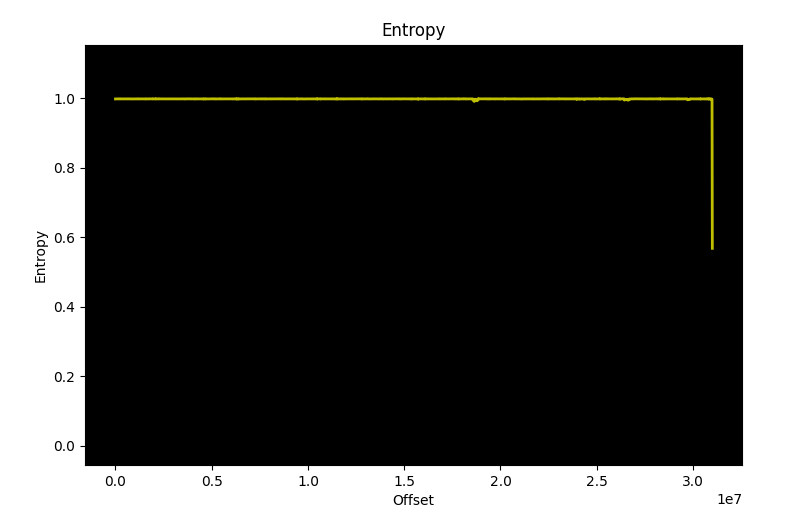
\includegraphics[scale=0.35]{r7000entropy.png}
    \caption{Gráfica de la entropía de la imagen firmware del Netgear R7000 generada por Binwalk.}
    \label{fig:binwalkEnt}
\end{figure}

\begin{figure}[H]
    \centering
    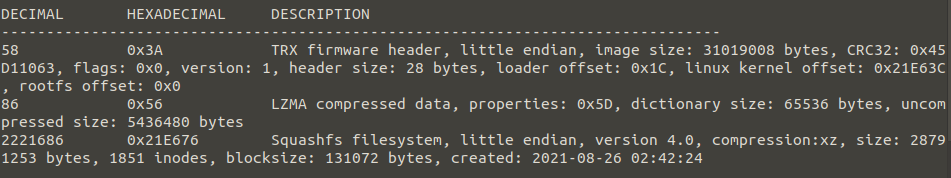
\includegraphics[scale=0.36]{r7000extraction.png}
    \caption{Extracción firmware Netgear R7000 usando Binwalk.}
    \label{fig:binwalkExt}
\end{figure}

\begin{figure}[H]
    \centering
    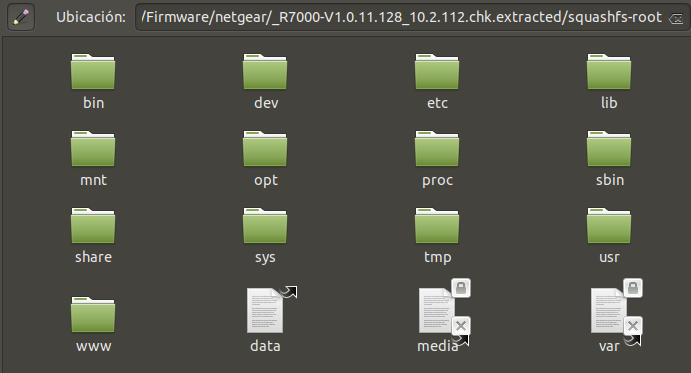
\includegraphics[scale=0.46]{r7000Squashfs.png}
    \caption{Sistema de archivos del Netgear R7000.}
    \label{fig:R7000squashfs}
\end{figure}

\begin{figure}[H]
    \centering
    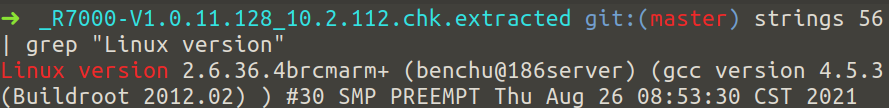
\includegraphics[scale=0.35]{r7000kernel.png}
    \caption{Versión del kernel utilizada por el R7000.}
    \label{fig:R7000kernel}
\end{figure}

Una vez extraído el firmware, podemos proceder a elegir un binario que nos resulte de interés para aplicarle fuzzing. Esto será
comentado en la siguiente sección.

\subsection{Introducción al experimento}
El experimento que va a ser realizado está basado en los descubrimientos realizados por el equipo de la firma de ciberseguridad GRIMM, publicados el
22 de Abril del 2022\cite{r7000GRIMM}. En su publicación, hacen una introducción a una vulnerabilidad detectada en el demonio UPNP presente en 
el firmware del Netgear R7000 en su versión 1.0.11.128 y anteriores. La vulnerabilidad se da concretamente en la funcionalidad de actualización de 
firmware proporcionada por el demonio UPNP y consiste en un buffer-overflow que puede llevar a ejecución remota de código (RCE) por parte de un usuario 
identificado en el sistema al proporcionar un paquete de actualización de firmware malicioso. Esto es posible debido a que la rutina de actualización 
al comprobar los headers confía en los tamaños especificados en la cabecera TRX\cite{firmwareFormat} incluida en el paquete de firmware proporcionado 
por el usuario para realizar operaciones de memoria. A continuación, aplican emulación full-system en QEMU con el objetivo de recrear la vulnerabilidad 
y diseñar una prueba de concepto de un firmware malicioso.\bigskip

El equipo de GRIMM identificó la vulnerabilidad mediante análisis estático de código haciendo uso de herramientas de decompilación como Ghidra\cite{Ghidra}.
Aunque se trata de una técnica efectiva, requiere de un experto cualificado que revise manualmente el código línea a línea y de un veredicto potencialmente 
incompleto. Como es lógico, no se trata de un procedimiento que pueda ser fácilmente escalable. Además, hacen uso de emulación full-system cuando solo desean
poner a prueba una pequeña parte de la funcionalidad del demonio. Es por ello que proponemos mejoras para ambos de los aspectos mencionados mediante la aplicación 
de técnicas alternativas. En primer lugar, respecto al procedimiento de identificación de la vulnerabilidad podemos hacer uso de fuzzing, realizando de forma 
automática mutaciones a la imagen del firmware que se proporciona a la rutina de actualización. Al aplicar fuzzing, posibilitamos la detección de vulnerabilidades 
similares a gran escala y ayudamos al revisor de código a evitar tener que analizar código superfluo pudiendo centrarse en analizar los crashes detectados por
el fuzzer, sabiendo ya que se trata de código problemático. En segundo lugar, podemos obtener una mejora de rendimiento sustituyendo la emulación full-system 
por el uso de técnicas basadas en Unicorn\cite{unicorn} que nos permitan instrumentar exactamente la rutina de actualización de firmware incluida en el 
demonio UPNP.\bigskip

En resumen, el objetivo del experimento es intentar identificar la misma vulnerabilidad pero haciéndolo a través de fuzzing, a la misma vez que comparamos el enfoque de 
emulación aplicado por el equipo de GRIMM con otras técnicas de emulación alternativas.

\subsection{Realización del experimento}
\subsubsection{Análisis del binario}
Comenzaremos por identificar el binario que implementa la funcionalidad del UPNP en el firmware y cargarlo en Ghidra\cite{Ghidra} para obtener una visión
decompilada o reconstruida del código original que nos permita encontrar la rutina de código que gestiona las actualizaciones del firmware. Para ello, 
accedemos al sistema de archivos que fue extraído del firmware previamente y abrimos con Ghidra el binario ubicado en ''usr/sbin/upnpd''. Una vez 
hecho esto, podemos guiar nuestra búsqueda por las cadenas de texto de mensajes de log presentes en el binario. Utilizando la funcionalidad de búsqueda 
de strings en Ghidra podemos buscar strings relacionadas con términos como ''firmware'', ''header'', ''update'' o similares. Dado que la vulnerabilidad 
se da a la hora de comprobar los headers del firmware, buscamos por ''header'' y rápidamente identificamos el string ''Header checksum error!!!'' 
siendo referenciado por dos funciones distintas (figura \ref{fig:R7000string}).

\begin{figure}[H]
    \centering
    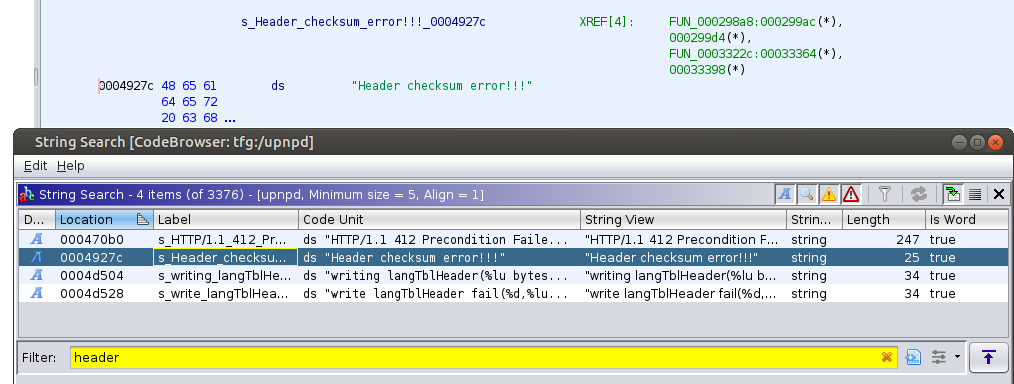
\includegraphics[scale=0.35]{r7000string.png}
    \caption{Resultados de la búsqueda de strings en Ghidra.}
    \label{fig:R7000string}
\end{figure}

Ambas funciones implementan aparentemente la misma lógica de parsing de la cabecera del firmware con la única diferencia de que ''FUN\_0003322c''
(figura \ref{fig:R7000decompilado}) contiene hardcodeado el modelo del dispositivo para compararlo con un valor incluido en el firmware. 
Ya que esta función parece destinada a nuestro modelo específico, será la función que usemos como objeto de pruebas más adelante y la apodaremos 
''check\_upd\_header''. Realizando un breve 
análisis del código decompilado, podemos observar que en la línea 17 se comprueba una cadena mágica para verificar que se trata de un firmware, 
en las líneas 29 y 30 se realizan operaciones con memoria que analizaremos más adelante y de la línea 34 a la 44 se llevan a cabo comprobaciones de que 
el firmware corresponda con el modelo de dispositivo en el que va a ser instalado.

\begin{figure}[H]
    \centering
    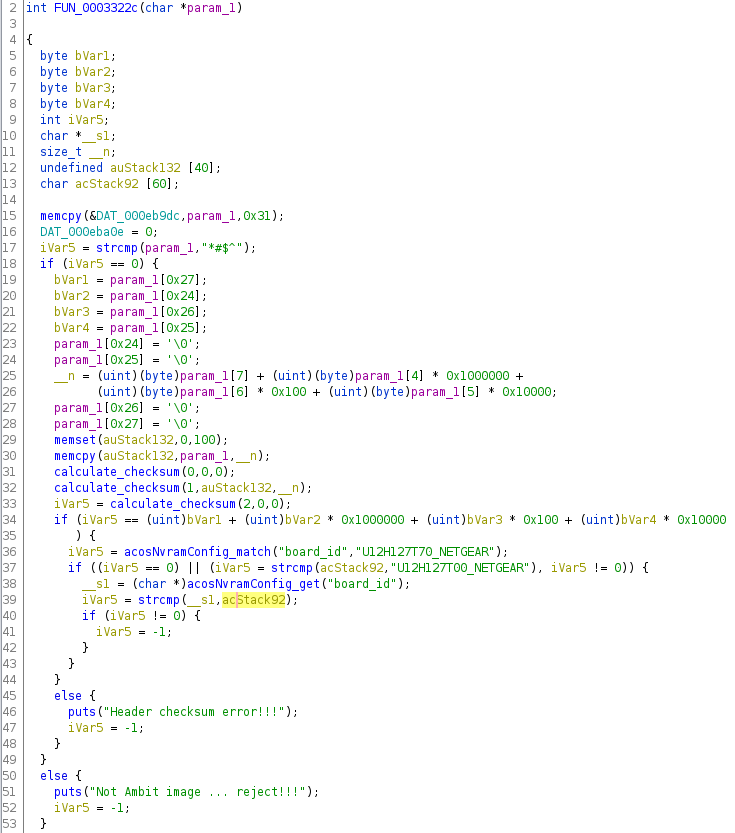
\includegraphics[scale=0.45]{r7000decompilado.png}
    \caption{Función del UPNP decompilada por Ghidra.}
    \label{fig:R7000decompilado}
\end{figure}

\subsubsection{Emulación del binario}
Es imprescindible conseguir emular el binario como paso previo a aplicar fuzzing sin disponer del dispositivo original. Para ello, como se ha comentado 
anteriormente pondremos a prueba tanto la metodología de emulación QEMU full-system propuesta por GRIMM en su artículo como una emulación mediante 
Qiling\cite{qiling} que en lugar de emular el demonio en su totalidad, instrumente el binario para ejecutar exclusivamente la función que hemos identificado 
en la sección anterior. Además, pondremos a prueba la efectividad de FirmAE\cite{Kim2020} para comprobar si pudiera proporcionar una mejor experiencia de 
emulación full-system en comparación con QEMU básico.

\paragraph{Qiling}
Para emular la función deseada con Qiling, aplicaremos la misma técnica que ha sido desarrollada en la prueba de concepto anterior, es decir, se harán uso 
de dos hooks para alterar el flujo de ejecución del código. El primer hook se ejecutará al llegar al punto de entrada del ejecutable y reemplazará el primer 
parámetro de la función (registro R0 según la convención de llamada a funciones en ARM32) con la dirección en hexadecimal de check\_upd\_header() para convertir 
la función en el main del programa. El segundo hook también sigue el mismo funcionamiento, dado que check\_upd\_header() solo recibe como parámetro un array 
de bytes representando el header del firmware, solo será necesario alocar manualmente los bytes que el script de Qiling haya leído de un archivo que se le 
pase por línea de comandos. En la figura \ref{fig:R7000flowchart} podemos observar el flujo de ejecución aplicando instrumentación 
dinámica con el script de Qiling.

\begin{figure}[H]
    \centering
    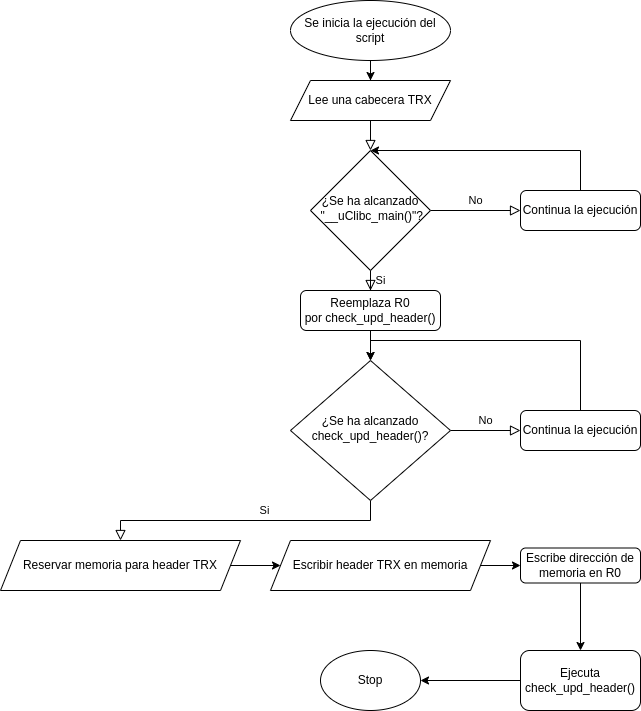
\includegraphics[scale=0.45]{r7000flowchart.png}
    \caption{Diagrama de flujo representando la instrumentación realizada sobre UPNP.}
    \label{fig:R7000flowchart}
\end{figure}

Para crear el script, empezamos consultando en Ghidra la dirección de la función ''\_\_uClibc\_main()'' y las direcciones de 
inicio y fin de la función target check\_upd\_header() para crear variables reconocibles en el script. Para el caso de este 
binario, las direcciones son las siguientes:

\begin{lstlisting}[language=python, caption=Declaración de constantes: Direcciones de interés en funciones., captionpos=b,
     frame=single, breaklines]
    TARGET_FUNC_ADDR    = 0x3322c   # Address of the function we are interested in
    TARGET_END_ADDR     = 0x33360   # End fuzzing when reaching this address
    LIBC_START_ADDR     = 0x0c460   # Address where __uClibc_main is being called
\end{lstlisting}

Gracias a la intuitiva API de Qiling, establecer los hooks es tan fácil como asociar la dirección de una instrucción del binario
con una función del script. También cabe mencionar que definiremos como ''rootfs'' la ruta al sistema de archivos extraído del
firmware previamente para que el enlazado dinámico de librerías se produzca correctamente. Definimos de la siguiente manera los
hooks y sus funciones asociadas.

\begin{lstlisting}[language=python, caption=Declaración de constantes: Direcciones de interés en funciones., captionpos=b,
    frame=single, breaklines]
    def libc_start_main_redirect(ql: Qiling, func_addr = TARGET_FUNC_ADDR):
    ql.reg.write("r0", func_addr)
    
    def indirect_write_reg_bytes(ql: Qiling, register_id, bytes):
        address = ql.mem.map_anywhere(len(bytes))
        ql.mem.write(address, bytes)
        ql.reg.write(register_id, address) # == (ql.reg.r0 = address) 

    def target_hook(ql: Qiling):    
        print("\n--------------\n")
        print("HOOK, PC: 0x%x" % ql.reg.arch_pc)
        print("Using", PAYLOAD, "as payload\n")
        indirect_write_reg_bytes(ql, "r0", PAYLOAD)
        print("\n--------------\n")
        
    def sandbox(path, rootfs, debug):    
        ql = Qiling(path, rootfs)
        ql.hook_address(libc_start_main_redirect, LIBC_START_ADDR)
        ql.hook_address(target_hook, TARGET_FUNC_ADDR)     
        ql.debugger = debug
        ql.run(end=TARGET_END_ADDR)

    ...
\end{lstlisting}

Tras crear el script, necesitaremos un sample de cabeceras de firmware para pasarle a este como parámetro y comprobar así
su funcionamiento. Para ello, simularemos un caso de actualización de firmware real, es decir, descargaremos el paquete de 
firmware correspondiente a la siguiente versión (1.0.11.128 -> 1.0.11.134) y extraeremos los mil primeros bytes de este ya que 
solo estamos interesados en las cabeceras y el inicio del fichero. DD permite hacer esto con la siguiente orden:

\begin{lstlisting}[language=bash, breaklines]
    $ dd if=R7000-V1.0.11.134_10.2.119.chk of=header134.chk count=1 bs=1K
\end{lstlisting}

Mirando el volcado en hexadecimal del fichero resultante (figura \ref{fig:R7000header}), saltan rápidamente a la vista dos de
los campos descritos anteriormente al tratar la estructura de una cabecera TRX y las comprobaciones previas que realiza 
check\_upd\_header(), el magic number al inicio del fichero con el valor ''*\#\$\textasciicircum'' y el modelo de dispositivo
para el que va destinada la actualización ''U12H270T00\_NETGEARHDR0''.

\begin{figure}[H]
    \centering
    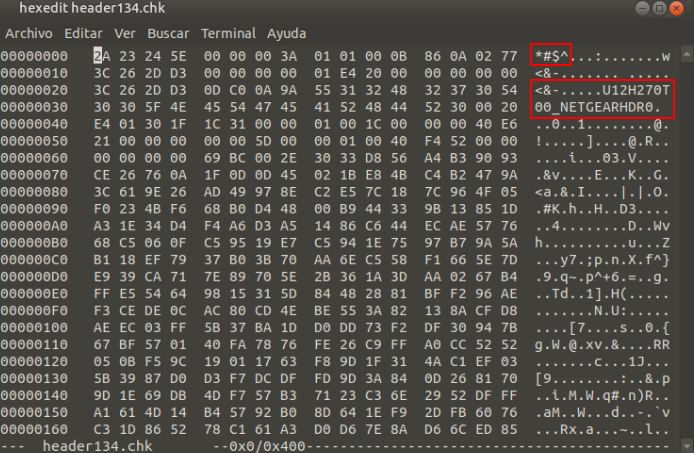
\includegraphics[scale=0.5]{r7000header.png}
    \caption{Representación hexadecimal del contenido del firmware.}
    \label{fig:R7000header}
\end{figure}

A continuación, podemos ejecutar el script y comprobar su funcionamiento. Al ejecutarlo pasando como parámetro 
''header134.chk'' (figura \ref{fig:R7000qiling}), observamos que los hooks se aplican correctamente y aunque la ejecución 
parece finalizar correctamente se muestran errores ENOENT debido a la ausencia de una NVRAM en ''/dev/nvram''. Esto se produce cuando la función emulada
intenta consultar en la NVRAM la variable ''board\_id'' para compararla con el string del modelo en el firmware comentado
anteriormente. Dado que no estamos emulando la NVRAM ni haciendo uso de librerías alternativas como nvram-faker\cite{nvram}
para interceptar las operaciones con este dispositivo, se producen errores al intentar consultar variables en este pero ya
que solo se utiliza para realizar la comparación de ambas cadenas, podemos ignorar los errores por el momento.

\begin{figure}[H]
    \centering
    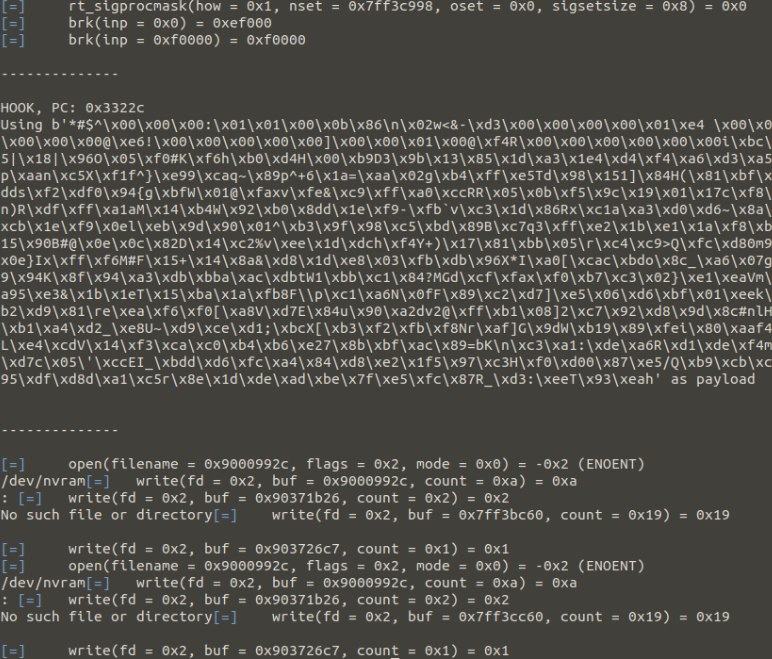
\includegraphics[scale=0.4]{r7000qiling.png}
    \caption{Resultado de la emulación de check\_upd\_header() con Qiling.}
    \label{fig:R7000qiling}
\end{figure}

Si probamos a modificar la cadena mágica del firmware y a pasárselo al script, comprobamos que efectivamente se avisa de que 
el fichero no se trata de una actualización de firmware válida (figura \ref{fig:R7000magic}), cancelando así el proceso de actualización si estuviéramos 
emulando el binario al completo.

\begin{figure}[H]
    \centering
    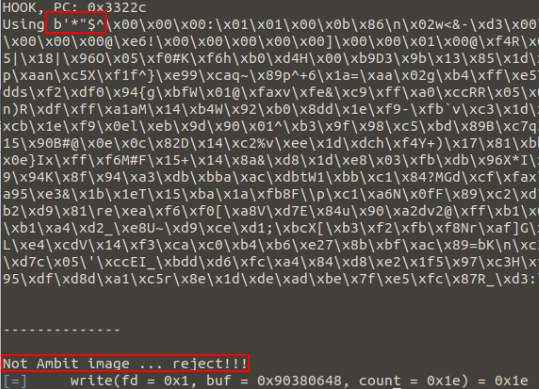
\includegraphics[scale=0.5]{r7000magic.png}
    \caption{Fallo al comprobar la cadena mágica en Qiling.}
    \label{fig:R7000magic}
\end{figure}

\paragraph{QEMU}
\paragraph{FirmAE}


\subsubsection{Aplicación de fuzzing}

\subsection{Resultados}
\subsection{Lecciones aprendidas}
